\newpage
\section{Prac 2.1 - OpenCL}
\label{sec:Prac2}

\subsection{Introduction}

This practical focuses on  developing an OpenCL kernel, using C++, that you can load, activate and send data back and forth to, from a C / C++ host application. The following quote, from Kronos \cite{opencl_khronos}, summarises what  OpenCL is:

\begin{quote}
    OpenCL™ (Open Computing Language) is the open, royalty-free standard for cross-platform, parallel programming of diverse processors found in personal computers, servers, mobile devices and embedded platforms. OpenCL greatly improves the speed and responsiveness of a wide spectrum of applications in numerous market categories including gaming and entertainment titles, scientific and medical software, professional creative tools, vision processing, and neural network training and inferencing. \cite{opencl_khronos}
\end{quote}

The main purpose of practical 2.1 is to show you how a typical OpenCL program would run by taking a step-by-step approach. Furthermore, this practical has to be completed \textbf{individually}.

\subsection{Requirements}
The Blue Lab PCs have all the required packages installed, but if you wish to run this practical on your own machine, you will need to install OpenCL as per the instructions on the Wiki - \href{http://wiki.ee.uct.ac.za/OpenCL}{http://wiki.ee.uct.ac.za/OpenCL}. Furthermore, you will have to install the appropriate SDK (software development kits) for the device you are planning to run the program on. The following links will direct to you to the appropriate websites explaining how to install the SDK for their respective devices.
\begin{itemize}
    \item Nvidia: \href{https://developer.nvidia.com/cuda-toolkit}{https://developer.nvidia.com/cuda-toolkit}
    \item Intel: \href{https://www.intel.com/content/www/us/en/developer/tools/opencl-sdk/choose-download.html}{https://www.intel.com/content/www/us/en/developer/tools/opencl-sdk/choose-download.html}
    \item AMD: \href{https://developer.amd.com/wordpress/media/2012/10/AMD_APP_SDK_InstallationNotes.pdf}{https://developer.amd.com/wordpress/media/2012/10/AMD_APP_SDK_InstallationNotes.pdf}
\end{itemize}

Lastly, all code required to start this practical is on the courses github repository \href{https://github.com/UCT-EE-OCW/EEE4120F}{https://github.com/UCT-EE-OCW/EEE4120F}.

\subsection{The Programming Model}
OpenCL uses a programming and memory model similar to OpenGL. The CPU must copy data to the GPU and then tell a kernel (OpenCL worker) to process the data. When the kernel is finished, the CPU can read back the result. This is an overly simplistic summary, the steps below will explain in more detail how this process takes place.


\subsection{Step by Step Explanation}
This step by step explanation works very closely to the code provided in the github repository, so please clone the repository if you have not already.

\subsubsection{Preparation}
Before, setting up the the main task for this practical you have to check what platforms (SDKs) you have installed on your host computer and determine what device you would like to run the program on. In order to do this the program platform.cpp has been given to you. This c++ program will be used to test if you have setup openCL correctly and then output the index's for the platforms installed on your host device.

After compiling and running the platform.cpp program you should get an output similar to the image below.

\begin{figure}[H]
\centering
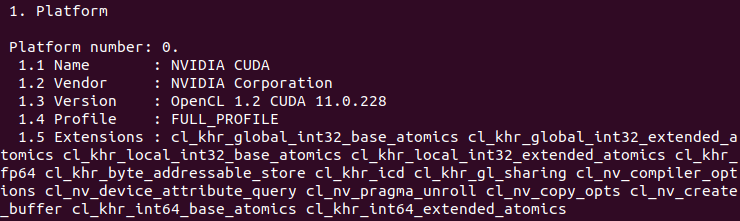
\includegraphics[width=0.6\columnwidth]{Figures/platformOutput.png}
\caption{Example Output of Platform.cpp}
\label{fig:platform}
\end{figure}

Take not of the the `platform number' because you will need this later in the practical.

The following steps will require you to open the main.cpp file and make the appropriate changes. The main.cpp file has sections of code missing which you will have to fill in, these sections are labeled 'TODO code' with the code numbers. Whilst, the manual below will be labeled similarly.
\subsubsection{Step 1}
OpenCL is a heterogeneous programming tool, which means you can program on different devices and differing platforms on the host computer. This in turn requires you to select the correct platform for the device you would like to run your program on. In order to select the platform you would like to use the following command is run. 
\begin{lstlisting}
cl_int clGetPlatformIDs(cl_uint num_entries,
					cl_platform_id *platforms, 
					cl_uint *num_platforms)
\end{lstlisting}

This function saves all available platforms in a list of type cl\_platform\_id with its pointer being set the argument *platforms. We can now select which device to use by indexing this list, with the platform number obtained when running the platform.cpp program. 

\begin{lstlisting}
//TODO: code 1
//Change index depending on the platform you want to use
cl_platform_id platform = platforms[0]; 
\end{lstlisting}

\subsubsection{Step 2}
After selecting your platform you need to choose the device that this platform will be utilizing. The following command allows you to do that.

\begin{lstlisting}
cl_int clGetDeviceIDs(cl_platform_id platform,
		cl_device_type device_type, 
		cl_uint num_entries, 
		cl_device_id *devices, 
		cl_uint *num_devices)
\end{lstlisting}
Similarly, to the clGetPlatformIDs() function, clGetDeviceIDs() saves the device id's to the cl\_device\_id variable that you enter as an argument as shown below. Also, note that you will have to indicate the type of device you are looking for and due to most computer only having one CPU and possible one GPU we set the num\_entries to 1. Resulting in your 'devices' variable containing only one device id, which is your GPU or CPU.

\begin{lstlisting}
\\TODO code 2
err = clGetDeviceIDs(platform, CL_DEVICE_TYPE_GPU, 1, &device, NULL);

OR

err = clGetDeviceIDs(platform, CL_DEVICE_TYPE_GPU, 1, &device, NULL);
\end{lstlisting}


\subsubsection{Step 3}
Often in OpenCL programs you have multiple devices all processing various aspects of the program. In this practical we are only dealing with a GPU or CPU. However, due to the heterogeneous nature of OpenCL, a context has to be created to house all available devices that the the program is planning on using. 

The following command creates a context with all the devices you are planning on using in the program, which you obtained in step 2.
\begin{lstlisting}
cl_context clCreateContext(cl_context_properties *properties,
					cl_uint num_devices,
					const cl_device_id *devices,
					void *pfn_notify(const char *errinfo, 
					const void *private_info, size_t cb, 
					void *user_data),
					void *user_data,cl_int *errcode_ret)
\end{lstlisting}

For this practical we are only using the one device obtained in step two and the following command has to be added to main.cpp.

\begin{lstlisting}
\\TODO code 3
cl_context context;
	context = clCreateContext(NULL, 1, &device, NULL, NULL, NULL);
\end{lstlisting}

\subsubsection{Step 4}
Now that the platforms and devices have been added to the context, the program we want to run on these devices need to be loaded into a buffer, as a string. So that we can isolate what we want to run on the various devices. The file used in this practical is, `OpenCL/Kernel.cl'.

\begin{lstlisting}
//TODO code 4
program_handle = fopen("OpenCL/Kernel.cl", "r");
\end{lstlisting}


\subsubsection{Step 5}
A program variable has to then be created from the source code obtained in step 4, essentially adding the program to the context. Note, you could have multiple programs each with their own program ID.
\begin{lstlisting}
cl_program clCreateProgramWithSource(cl_context context,
							cl_uint count, 
							const char **strings, 
							const size_t *lengths, 
							cl_int *errcode_ret)	
\end{lstlisting}

\begin{lstlisting}
//TODO code 5
cl_program program = clCreateProgramWithSource(context, 1, 
                        (const char**)&program_buffer, &program_size, NULL);
\end{lstlisting}

\subsubsection{Step 6}
In order for our program to run on the device we want, the program has to be compiled for that specific device. The function clBuildProgram() compiles your selected program for a specific device, using the device IDs obtained in step 2.

\begin{lstlisting}
cl_int clBuildProgram(
    cl_program program,
    cl_uint num_devices,
    const cl_device_id* device_list,
    const char* options,
    void (CL_CALLBACK* pfn_notify)(cl_program program, void* user_data),
    void* user_data);
\end{lstlisting}

\begin{lstlisting}
\\TODO code 6
cl_int err3= clBuildProgram(program, 0, NULL, NULL, NULL, NULL);
\end{lstlisting}

\subsubsection{Step 7}
Now that the program has been compiled for the device you want to run it on. You need to select what section of this program that you have compiled, you want to run on the selected device. These sections of code are referred to as kernels, and are represented as functions in the 'cl\_program' setup in step 6. If you look in the file OpenCL/Kernel.cl you will see a function called HelloWorld, this is the kernel for this practical.

\begin{lstlisting}
cl_kernel clCreateKernel(cl_program program,
	                        const char* kernel_name,
	                        cl_int* errcode_ret);
\end{lstlisting}

\begin{lstlisting}
\\TODO code 7
cl_kernel kernel = clCreateKernel(program, "HelloWorld", &err);
\end{lstlisting}

\subsubsection{Step 8}
Currently, we now have all the platforms, devices and kernels setup for the practical. However, the kernels needs a way to get from the host to your selected device (ie GPU or CPU). A command queue is required to facilitate this process.

\begin{lstlisting}
cl_command_queue clCreateCommandQueueWithProperties(cl_context context,
                                            cl_device_id device,
                                            const cl_queue_properties* properties,
                                            cl_int* errcode_ret);
\end{lstlisting}

For this practical the queue that you have to setup is between the host and the device you have selected. This queue is created with the following command.

\begin{lstlisting}
\\TODO code 8
cl_command_queue queue = clCreateCommandQueueWithProperties(context, device, 
                                                            0, NULL);
\end{lstlisting}

\subsubsection{Step 9}
Note the queue only allows for kernels to be sent, which is contains only the program that must be run for each work item. So we need to setup data buffers to allow for communication between devices. Which is our case is communication between the host and target device. 

This can be done with the clCreateBuffer() function which sets up shared memory between devices that both the host and target device can access. This has to be done as your GPU by default uses its VRAM, while the host will use the computers RAM, and these memory units are completely separate, so the GPU can't access the RAM and the host CPU can't access the VRAM. Therefore, the memory blocks we are setting up now, are block's of memory where both devices can access them.

\begin{lstlisting}
	cl_mem clCreateBuffer(cl_context context,
				cl_mem_flags flags,
				size_t size,
				void* host_ptr,
				cl_int* errcode_ret);
\end{lstlisting}

For this practical you need to setup 3 buffers, the first 2 buffers are only one integer in size and will allow for the target device to access these arguments. Note in the code below that your target device may read these buffers but may not alter them.

The last buffer will be your output buffer used to store the outputs from your kernel, so that the host can retrieve what the kernels calculated.

\begin{lstlisting}
\\TODO code 9.2
argument1_buffer = clCreateBuffer(context, 
            CL_MEM_READ_ONLY | CL_MEM_COPY_HOST_PTR, 
            sizeof(int), &argument1, &err);

argument2_buffer = clCreateBuffer(context, 
            CL_MEM_READ_ONLY | CL_MEM_COPY_HOST_PTR, 
            sizeof(int), &argument2, &err);
	
output_buffer = clCreateBuffer(context, 
            CL_MEM_READ_WRITE | CL_MEM_COPY_HOST_PTR, 
            global_size*local_size*sizeof(int), output, &err);
  
\end{lstlisting}

Furthermore, if you look at the output buffer, we set the size to global\_size*sizeof(int), this is due to the fact that each work item needs to have it own output of one interger in size. 

Therefore, before setting the memory buffers we need to determine how many work items and work groups we want for the program. So we set the following variables that contain the required information, which we will use at a later stage.

\begin{lstlisting}
\\TODO step 9.1
size_t global_size = 16; //total number of work items
size_t local_size = 4; //Size of each work group
cl_int num_groups = global_size/local_size; //number of work groups needed
\end{lstlisting}

\subsubsection{Step 10}
In order for our target device to utilize the memory blocks created in step 9, we have to add arguments to the kernel, giving the kernel the pointers to the blocks of memory. The clSetKernelArg() function links these memory blocks to the kernel. Note, when looking at the OpenCL/Kernel.cl file you will see the same arguments needed to run the kernel HelloWorld.

\begin{lstlisting}
cl_int clSetKernelArg (cl_kernel kernel, 
                        cl_uint arg_index, 
                        size_t arg_size, 
                        const void *arg_value)
\end{lstlisting}

In this practical we have setup 3 memory blocks, hence we need 3 kernel arguments as shown below.

\begin{lstlisting}
\\TODO step 10
clSetKernelArg(kernel, 0, sizeof(cl_mem), &argument1_buffer);
clSetKernelArg(kernel, 1, sizeof(cl_mem), &argument2_buffer);
clSetKernelArg(kernel, 2, sizeof(cl_mem), &output_buffer);

\end{lstlisting}


\subsubsection{Step 11}
Finally, we can now deploy the kernels to the target device using the clEnqueueNDRangeKernel() function and set the number of work items per work groups. The work items each run the kernel.cl file and can only access memory from other work items in the same group.

\begin{lstlisting}
 cl_int clEnqueueNDRangeKernel (cl_command_queue command_queue, 
						cl_kernel kernel, 
						cl_uint work_dim, 
						const size_t *global_work_offset, 
						const size_t *global_work_size, 
					    const size_t *local_work_size, 
						cl_uint num_events_in_wait_list, 
						const cl_event *event_wait_list, 
						cl_event *event)
\end{lstlisting}

For this practical we have already setup the number of work items (global\_size) and work groups, which we set in 9.1, so we just deploy the kernels as follows.

\begin{lstlisting}
//TODO code 11
cl_int err4 = clEnqueueNDRangeKernel(queue, kernel, 1, NULL, 
                &global_size, &local_size, 0, NULL, NULL); 
\end{lstlisting}    

\subsubsection{Step 12}
After the kernels have run, we now want the host to read from the output memory buffer, using the following command.

\begin{lstlisting}
//read from a buffer object to host memory
cl_int clEnqueueReadBuffer(
    cl_command_queue command_queue,
    cl_mem buffer,
    cl_bool blocking_read,
    size_t offset,
    size_t size,
    void* ptr,
    cl_uint num_events_in_wait_list,
    const cl_event* event_wait_list,
    cl_event* event);
    
//write to a buffer object from host memory
cl_int clEnqueueWriteBuffer(
    cl_command_queue command_queue,
    cl_mem buffer,
    cl_bool blocking_write,
    size_t offset,
    size_t size,
    const void* ptr,
    cl_uint num_events_in_wait_list,
    const cl_event* event_wait_list,
    cl_event* event);
\end{lstlisting}

In this practical we only need the host to read from the output buffer object, as shown below.

\begin{lstlisting}
\\TODO Step 12
err = clEnqueueReadBuffer(queue, output_buffer, CL_TRUE, 0, 
                        sizeof(output), output, 0, NULL, NULL);
\end{lstlisting}


\subsubsection{Step 13}
The last step is not actually part of the OpenCL process but rather just checking that the output received by the host is the same as the outputs calculated by the kernels.

\begin{lstlisting}
printf("\nOutput in the output_buffer \n");
	for(int j=0; j<global_size; j++) {
		printf("element number:%i \t Output:%i \n",j ,output[j]);
	}
\end{lstlisting}

\subsection{Kernel Creation}
Provided that you completed the Step by Step Explanation correctly when running the program you should get the following output, where each work item prints `Hello World'. Notice that the output value from step 13, are random numbers because the kernel has not updated the output buffer in any way. Therefore, the host's output will be whatever values were in those memory addresses before the program ran. 

\begin{figure}[H]
\centering
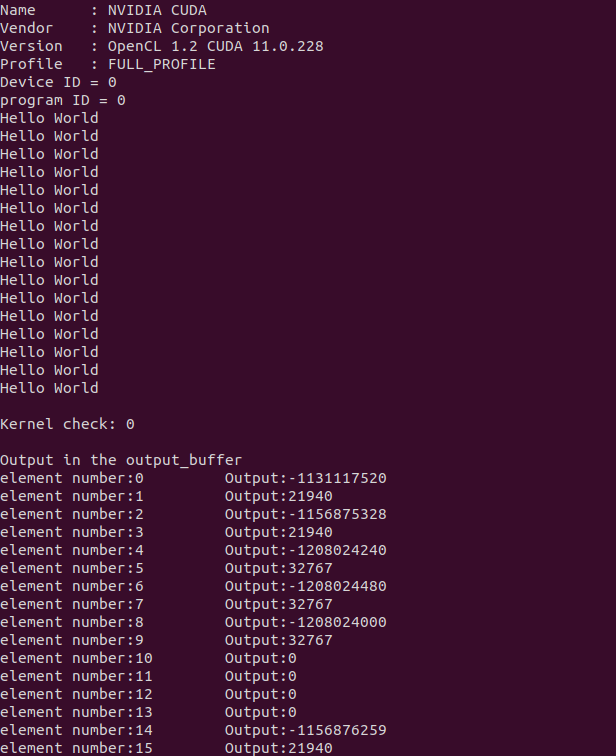
\includegraphics[width=0.6\columnwidth]{Figures/helloWorld.png}
\caption{Hello World Example Output}
\label{fig:Hello World}
\end{figure}

The final task for this practical is to edit the OpenCL/Kernel.cl file to complete the following tasks.

\subsubsection{Task 1}
Perform a basic numeric calculation that utilizes all the arguments for the kernel. The required calculation is given below. \newline
\newline
\begin{math} 
output[pos] = work Item Number x argument 1 + argument 2
\end{math}

\subsubsection{Task 2}
Print the work item, work group, arguments and output values, as follows.

\begin{figure}[H]
\centering
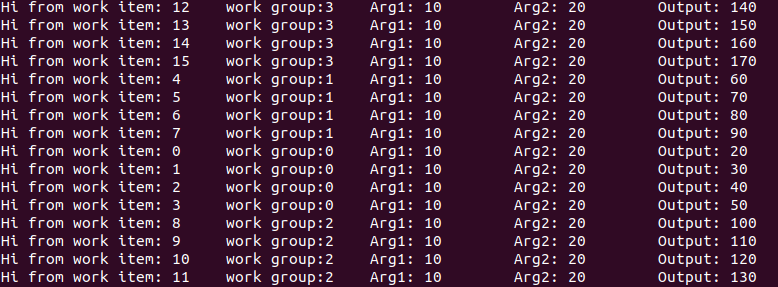
\includegraphics[width=0.9\columnwidth]{Figures/workItemOutput.png}
\caption{Expected Output}
\label{fig:Expected 1}
\end{figure}

\subsubsection{Task 3}
For the final task you have to add the output values of all the work items in each work group. 

In order to solve this issue consider isolating one work item, with an if statement, from each work group. This work item can then iterate through all the work items in the work group and add up each of their output values. Furthermore, make use of the barrier function that stops work items from continuing until all the work item in the group reach this barrier point. 

\begin{figure}[H]
\centering
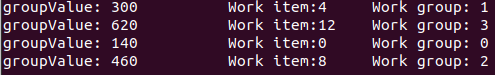
\includegraphics[width=0.9\columnwidth]{Figures/groupValues.png}
\caption{Expected Output}
\label{fig:Expected 2}
\end{figure}

\subsection{Submission}
For the final submission, submit your code in a zipped file labeled as follows `Prac2\_1\_STUDENTNUMBER'. The zipped file should contain the following files:
\begin{enumerate}
    \item main.cpp
    \item platforms.cpp
    \item OpenCL/Kernel.cl
    \item Any other compiled files
\end{enumerate}

\begin{table}[H]
\centering
\caption{Prac 2.1 Marking Guide}
\label{tbl:Prac2Marks}
\begin{tabular}{|l|l|r|}
\hline
\textbf{Aspect} & \textbf{Description} & \multicolumn{1}{l|}{\textbf{Mark Allocation}} \\ \hline
Main.cpp & &  \\ \hline
 & Steps & 13 \\ \hline
Kernel.cl & &  \\ \hline
 & Initial Calculation & 1 \\ \hline
 & Print Output & 2 \\ \hline
 & Work Group Total & 4 \\ \hline
TOTAL &  & 20 \\ \hline
\end{tabular}
\end{table}



